\chapter{Experimental Results}

\section{Setup}

\subsection{Tooling}

\subsection{Metric}

\subsection{Validation}

\subsection{Error Analysis}

\section{Results}

The metric used to evaluate the effectiveness of our models is the standard Area Under the ROC Curve (AUC), as adopted by \cite{abs-1807-01631}. Like \cite{CelonaM17}, we also used the leave-one-out method for cross validation and relevant hyper-parameters were found using a further internal comparison. The results reported are the average of the 15 runs, which are used to assess the overall performance of the models. Two variations of data augmentation intensity are also reported.

\begin{figure}[h!tp]
    \centering
    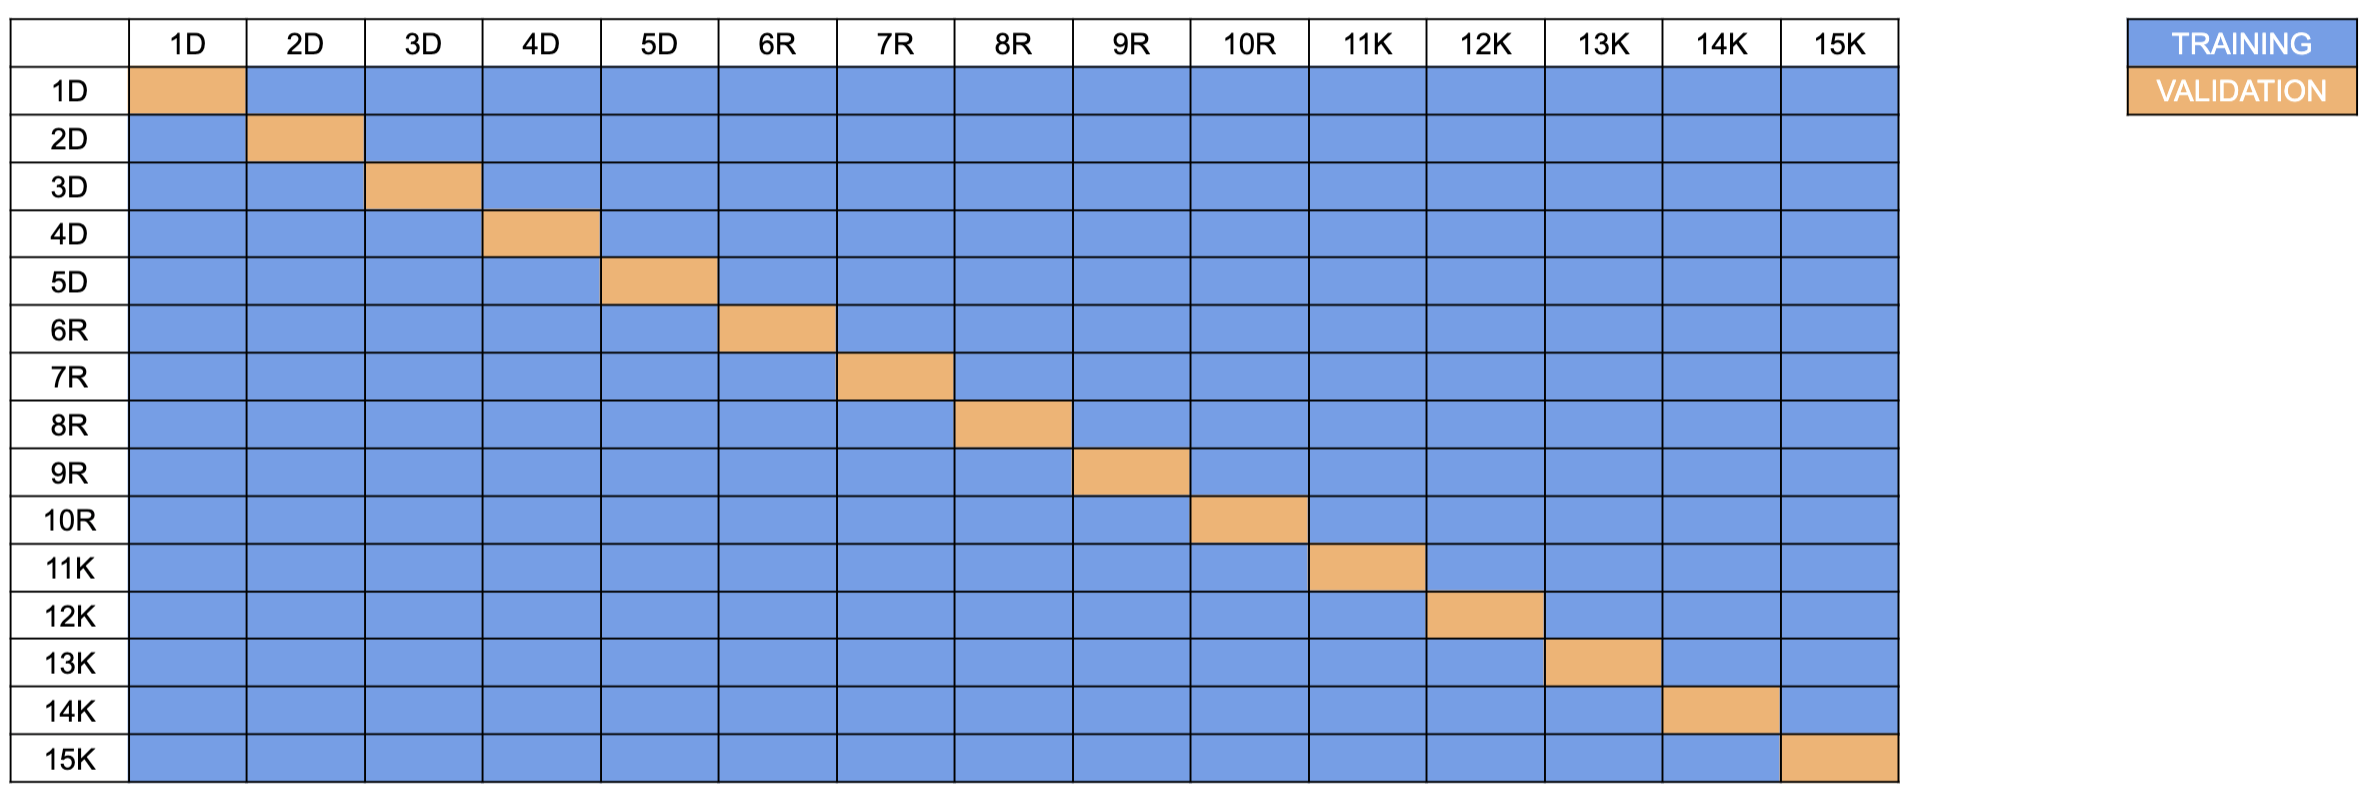
\includegraphics[width=1\textwidth]{imgs/chap4_validation.png}
    \caption{Leave-one-out validation process}
    \label{fig:validation}
\end{figure}

\begin{table}[htbp]
\centering
\caption{AUROC numbers for different network architectures and data augmentation intensity. The number in bold indicate the best approach on average in the validation process.}
\label{tab:results}
\begin{tabular}{lcc}
\hline
\multicolumn{1}{c}{}               & Mean           & Std            \\ \hline
VGG16 + Medium Data Augmentation   & 0.767          & 0.200          \\
VGG16 + Strong Data Augmentation   & 0.797          & 0.150          \\
VGGFace + Medium Data Augmentation & \textbf{0.884} & \textbf{0.119} \\
VGGFace + Strong Data Augmentation & 0.867          & 0.154          \\ \hline
\end{tabular}
\end{table}

\begin{figure}[htbp]
    \centering
    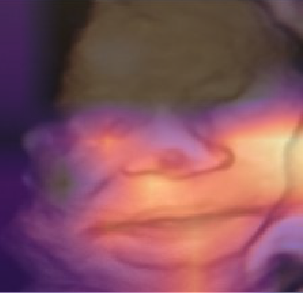
\includegraphics[width=0.4\textwidth]{imgs/chap4_gradcam.png}
    \caption{Grad-CAM heatmap for interpretability}
    \label{fig:gradcam}
\end{figure}

We have used the Grad-CAM \citep{SelvarajuCDVPB17} for interpretability, which is capable of creating a heatmap on the image with the fetures that were most relevant for the networks decision. An example can be seen on Figure \ref{fig:gradcam}.

